\documentclass{beamer}
\usepackage[spanish]{babel}
\usepackage[utf8]{inputenc}
\usepackage{graphicx}
\graphicspath{ {./images/}}

\usetheme{Madrid}
\usecolortheme{default}

%------------------------------------------------------------
%This block of code defines the information to appear in the
%Title page
\title[PC1 Estadistica Aplicada] %optional
{Aplicacion de tecnicas de estimacion y prueba de hipotesis}

\subtitle{
  Caso: tendencias socio-economicas de algunas
  lineas de carrea de Ingenieria de sistemas
}

\author % (optional)
{
  Alvarez \and Bautista \and Burga \and
  Casanova \and  Cuyate
}

\institute
{
  Facultad de Ingenieria Industrial y de Sistemas\\
  \textbf{Universidad Nacional de Ingenieria}
}

\date
{Octubre 2022}

% \logo{\includegraphics[height=1cm]{overleaf-logo}}

%End of title page configuration block
%------------------------------------------------------------

%------------------------------------------------------------
%The next block of commands puts the table of contents at the
%beginning of each section and highlights the current section:

\AtBeginSection[]
{
  \begin{frame}
    \frametitle{Tabla de Contenido}
    \tableofcontents[currentsection]
  \end{frame}
}
%------------------------------------------------------------


\begin{document}

%The next statement creates the title page.
\frame{\titlepage}


%---------------------------------------------------------
%This block of code is for the table of contents after
%the title page
\begin{frame}
\frametitle{Tabla de Contenido}
\tableofcontents
\end{frame}
%---------------------------------------------------------

\section{Problema}

\begin{frame}
\frametitle{Problematica}

\begin{itemize}
    \item Empiricamente se observa que en el mundo la precarizacion del trabajo
se acrecenta cada vez mas, de igual modo con la evolucion
    de personas casadas y los salarios promedio de los jovenes
    \item Con motivo de generar informacion util para la prediccion de estas tendencias
socio-economicas se ha procedio a realizar un analisis estadistico sobre
9 hipotesis planteadas

\end{itemize}
\end{frame}



%---------------------------------------------------------
\section{Objetivos}

%---------------------------------------------------------
\begin{frame}

\frametitle{Objetivos del trabajo}

\begin{alertblock}{General}
  Generar informacion relevante para la prediccion de tendencias
  socio-economicas en el mundo tomando como referencia datos
  provenientes de distintos paises.
\end{alertblock}
\end{frame}

\begin{frame}
\frametitle{Hipotesis especificas}

\begin{columns}
\column{0.5\textwidth}

  \begin{itemize}
      \item La distribucion de ingresos de  sigue
        la ley normal
      \item La distribución de ingresos de los trabajadores en software
        no sigue una distribución exponencial
      \item Las distribuciones de Delhi y Bangalore provienen de la
        misma poblacion
  \end{itemize}

\column{0.5\textwidth}

  \begin{itemize}
      \item En paises desarrollados existe una mayor cantidad
        de mujeres con puestos de trabajos relacionados a ingenieria que en paises en via
        de desarrollo
      \item Los cientificos de datos poseen un mejor distribucion de ingresos
        que los ingenieros de datos
      \item El sector \textit{(publico / privado)} al que pertenece un trabajador
        es causa de la diferencia de salarios
  \end{itemize}
\end{columns}
\end{frame}

%---------------------------------------------------------

\begin{frame}
\frametitle{Hipotesis especificas}
  \begin{itemize}
      \item Las personas que trabajan una cantidad de horas superior a
        la media tienen una mejor destribucion de ingresos que aquellas
        que no lo hacen
      \item Las personas de mediana edad poseen una mejor distribucion
        de ingreso que las personas jovenes
      \item El promedio de ingresos de la poblacion mexicana es mayor
        que la peruana
  \end{itemize}

  \textbf{Cada hipotesis tiene asociado el objetivo de comprobar
  o rechazar la suposicion}

\end{frame}

%---------------------------------------------------------


%---------------------------------------------------------
\section{Importancia de los objetivos}

\begin{frame}
  \textit{\textbf{
    Sobre los demas objetivos en general
  }}
  \newline

  Se consideraron las hipotesis de tal forma que brinde
  información relevante para el análisis del mercado laboral
  para los egresados de la carrera de \textit{Ingenieria de
  sistemas}

\end{frame}


\begin{frame}
  \textbf{\textit{
    Acerca de la forma de las distribuciones
  }}

  Antes de realizar cualquier tecnica de inferencia es necesario conocer
  la forma de las distribuciones, incluso antes de analizar la varianza

  \textbf{
    Sobre el analisis a realizar
  }

  Si bien se puede realizar \textbf{ANOVA} \footnotemark para cualquier distribucion
  las tecnicas de test parametricos requieren de la normalidad para admitir un error de
  tipo 1 del \text{5\%}

  \footnotetext[1]{\textit{Analysis of Variance}}


\end{frame}

%---------------------------------------------------------


\section{Resultados y Conclusiones}

\begin{frame}
  \frametitle{Hipotesis 1}
  \begin{figure}[t]
    \caption{Data sin estandarizar}
    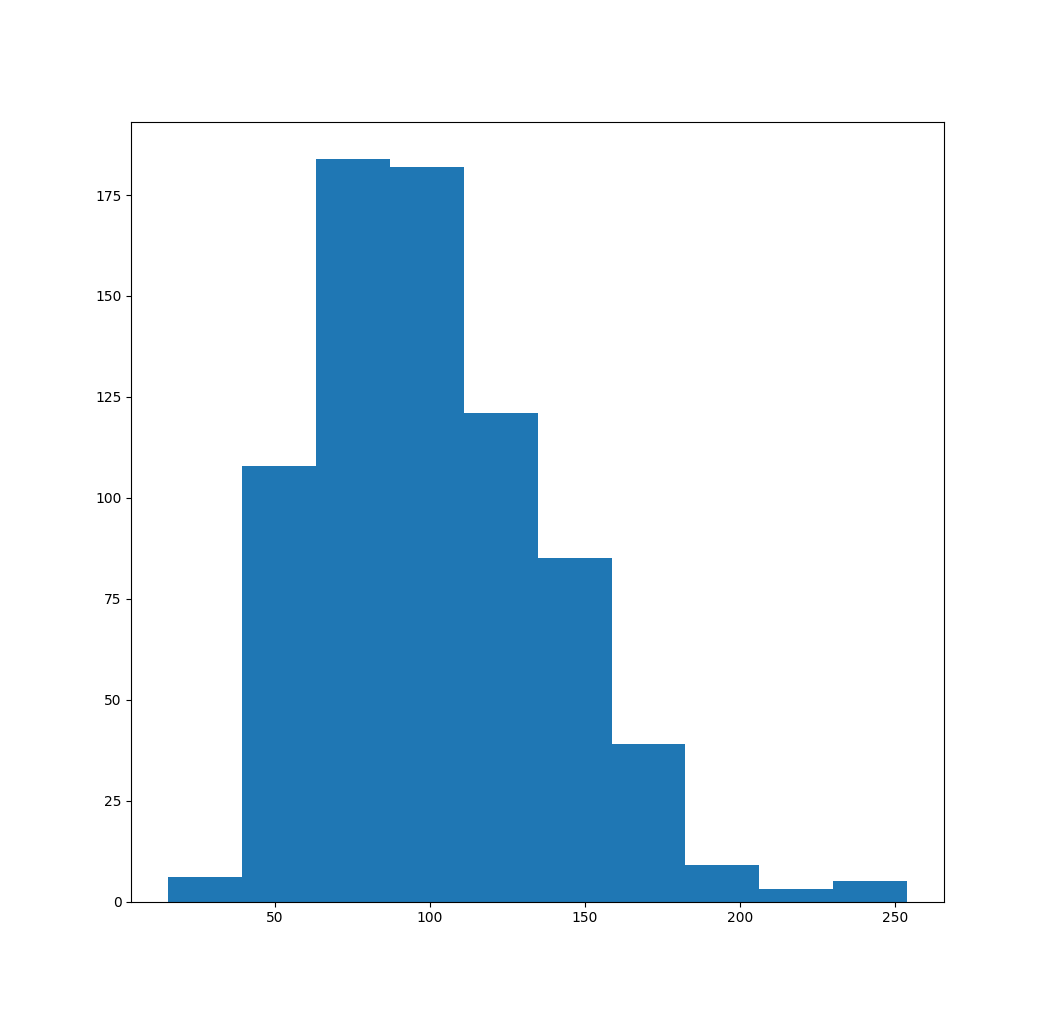
\includegraphics[width=5cm]{Figure_1.png}
  \end{figure}

\end{frame}

\begin{frame}
\frametitle{Hipotesis 1}
\begin{figure}[t]
  \caption{Data estandarizada y sin outliers}
  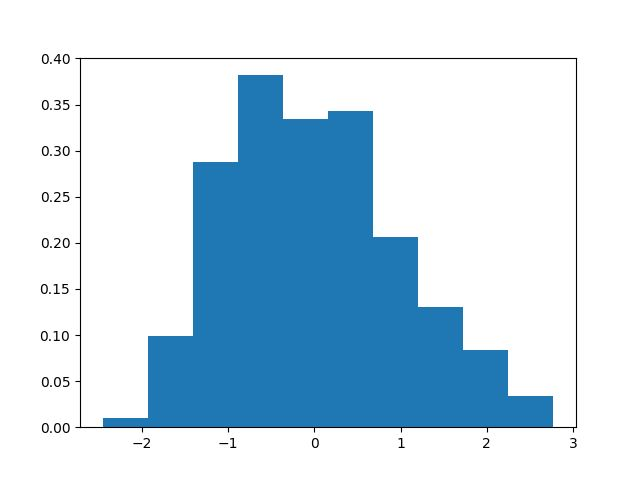
\includegraphics[width=6cm]{data_sin_outliers.jpeg}
\end{figure}
  \textbf{Puede parecer una distribucion Normal}

\end{frame}

\begin{frame}
\frametitle{Hipotesis 1}
\begin{figure}[t]
  \caption{Grafica Q-Q}
  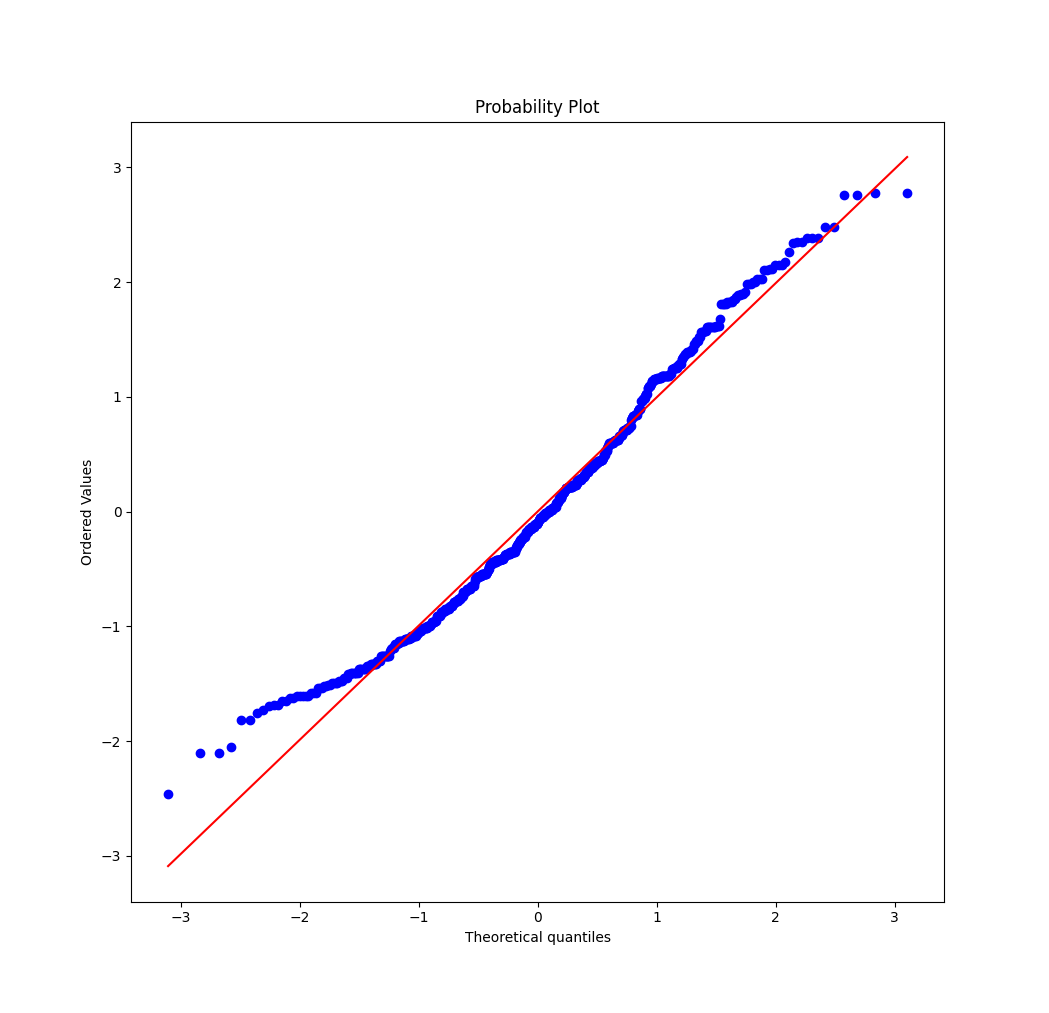
\includegraphics[width=6cm]{grafiaq-q.png}
\end{figure}

  \textbf{Se aleja de la distribucion normal}
\end{frame}

\begin{frame}

  Se aplicó el test de \textit{Jarque-Bera}, para comprobar si la muestra
  presenta una \textbf{curtosis} y \textbf{asimetria} correspondientes
  a una ley normal.

  El estadistico de \textit{Jarque Bera} es asintoticamente un estimador de
  una \textit{Chi-Cuadrado} (${\chi_n ^ 2}$) y toma como hipotesis nula que los datos de la
  muestra siguen la ley normal

  \begin{alertblock}{Test de Jarque-Bera}
    \[\textbf{JB} = \frac{n}{6}(S^2 +\frac{1}{4}(K - 3)^3)\] Siendo \textit{n} los grados de libertad
  \end{alertblock}

  \begin{block}{Estimadores de momentos centrales}
    \begin{itemize}
        \item Tercer Momento Central
          \[S = \frac{\hat{\mu}_3}{\hat{\sigma}^3}\]

        \item  Cuarto Momento Central
         \[K = \frac{\hat{\mu}_4}{\hat{\sigma}^4}\]
    \end{itemize}
  \end{block}
\end{frame}

\begin{frame}
  Adicionalmente, se usara el test de \textit{Kolmogorov-Smirnov}, donde se plantea
  que la distribucion de ingresos en la poblacion de ciencia de datos
  no sigue la ley normal y se comparará con la funcion acumulada teoria
  de esta

  \[H_0: \textrm{La distribucion de ingresos \textbf{NO sigue} la ley normal}\]
  \[H_1: \textrm{La distribucion de ingresos \textbf{SIGUE} la ley normal}\]

\end{frame}

\begin{frame}
\frametitle{Conclusiones hipotesis 1}
  El test K-S y el de Jarque-Bera muestran los siguientes p-values.
  \begin{figure}[t]
        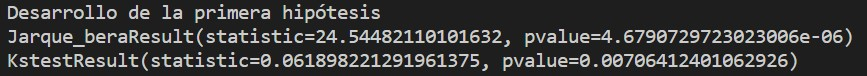
\includegraphics[width=12cm]{p-val-1.jpg}
    \end{figure}
    \begin{figure}[t]
          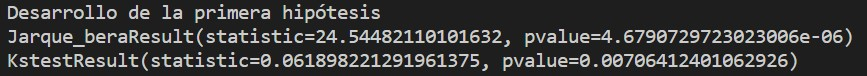
\includegraphics[width=12cm]{p-val-1.jpg}
      \end{figure}
    \end{frame}



\begin{frame}
\frametitle{Hipotesis 2}

\begin{figure}[h]
  \caption{Distribución de ingresos de ingenieros de
  software en la India}
  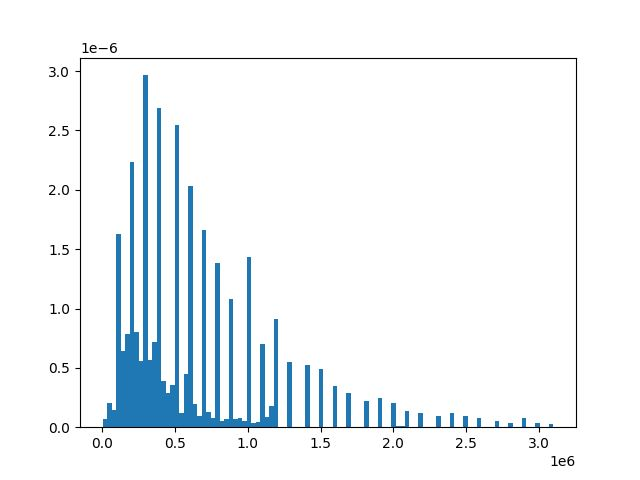
\includegraphics[width=6cm]{distribucion_ingresos_sw.jpeg}
\end{figure}

  se puede notar como existen \textit{2 grupos en la poblacion}
\end{frame}

\begin{frame}
  \frametitle{Distribución de los trabajadores en software}
  \alert{Aplicacion del test \textbf{Kolmogórov-Smirnov}}

  En este caso se va a comprar la funcion de distribucion acumulada observada
  con la de la distribucion teoria de una exponencial

\end{frame}

\begin{frame}
  \frametitle{Separando grupos aparentes}
  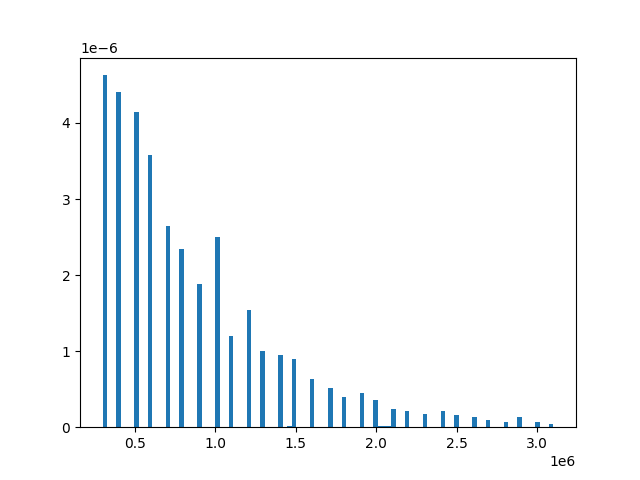
\includegraphics[width=8cm]{procesado.png}

\end{frame}

\begin{frame}
  \frametitle{Ajustando Curva}
  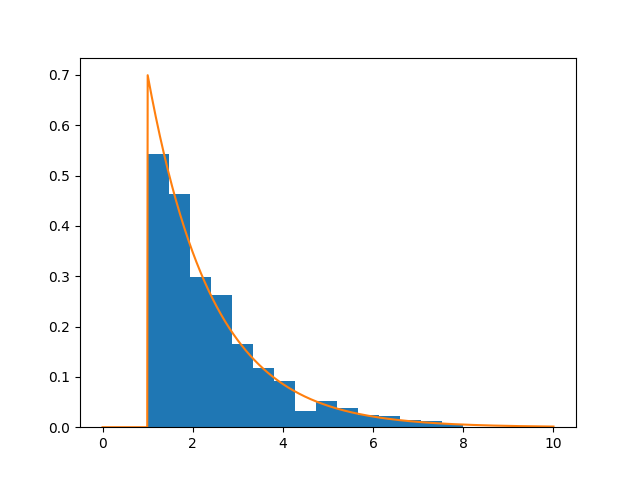
\includegraphics[width=8cm]{hip2/ajustando_curva.png}

\end{frame}

\begin{frame}
  \frametitle{Funciones acumuladas}
  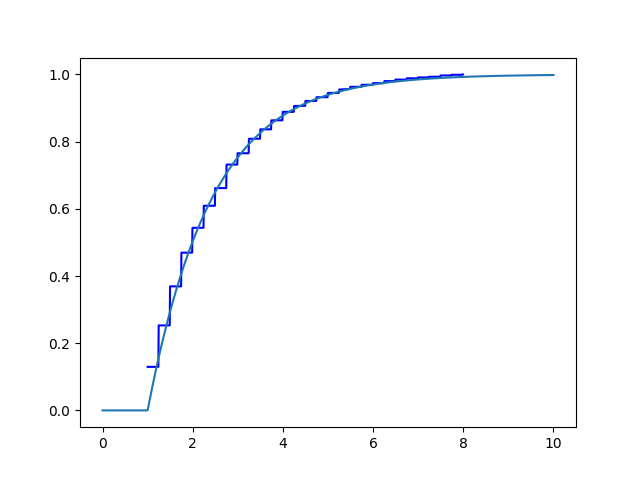
\includegraphics[width=8cm]{hip2/acumuladas.png}

\end{frame}

\begin{frame}
  \frametitle{Grafico P-P}
  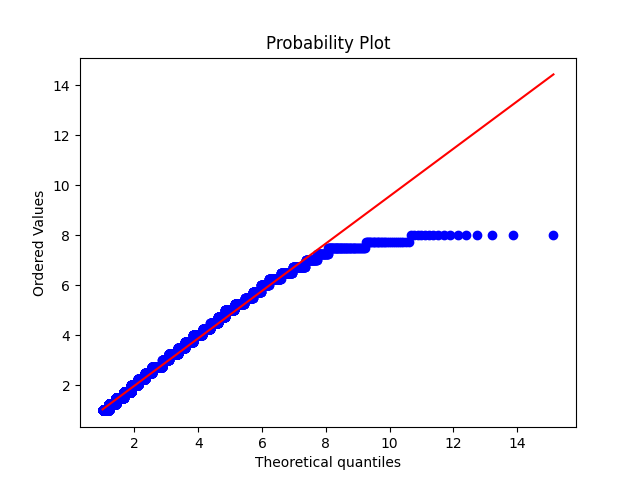
\includegraphics[width=8cm]{hip2/grafico_pp.png}
\end{frame}

\begin{frame}
  \frametitle{Conclusiones}
  De acuerdo al p-value obtenido no se puede rechazar la hipótesis nula
  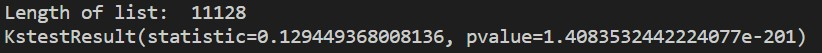
\includegraphics[width=9cm]{hip2/p-val.jpg}
\end{frame}

\begin{frame}
  \frametitle{Hipotesis 3}

  Se aplicó el test de \textit{Kruskal-Wallis} con la finalidad de:

  \begin{itemize}
      \item Verificar si las muestras de Delhi y Bangalore provienen de poblacines
        distinteas
  \end{itemize}

  Para esto se realizo un procedimiento similar al de la hipotesis anterior

  \begin{alertblock}{Consideracines del test}
    El test de Kruskal-Wallis es el sustituto no parametrico del
    \textit{"One way ANOVA"}, en el cual se necesita un factor independiente
  \end{alertblock}
\end{frame}

\begin{frame}
  \frametitle{Comparacion de salarios DC y DI}
  \[{X_1}: \textrm{Salario de cientifico de datos} \rightarrow \overline{X_1} = 1061.79389312977, {\sigma_1}^2 = ?\]
  \[{X_2}: \textrm{Salario de ingeniero de datos} \rightarrow \overline{X_1} = 916.603773584, {\sigma_2}^2 = ?\]
\begin{figure}[t]
  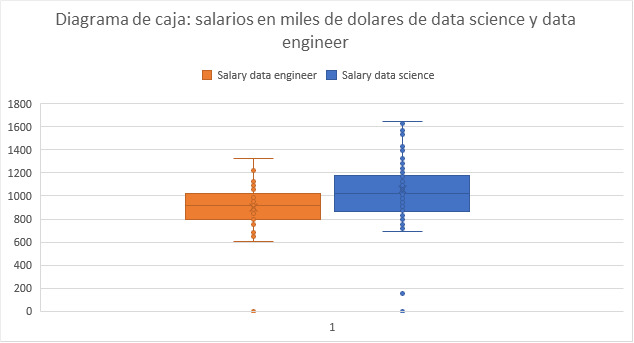
\includegraphics[width=6cm]{cajas1.jpeg}
\end{figure}
\end{frame}

\begin{frame}
  \frametitle{Test de hipotesis}
\begin{figure}[t]
    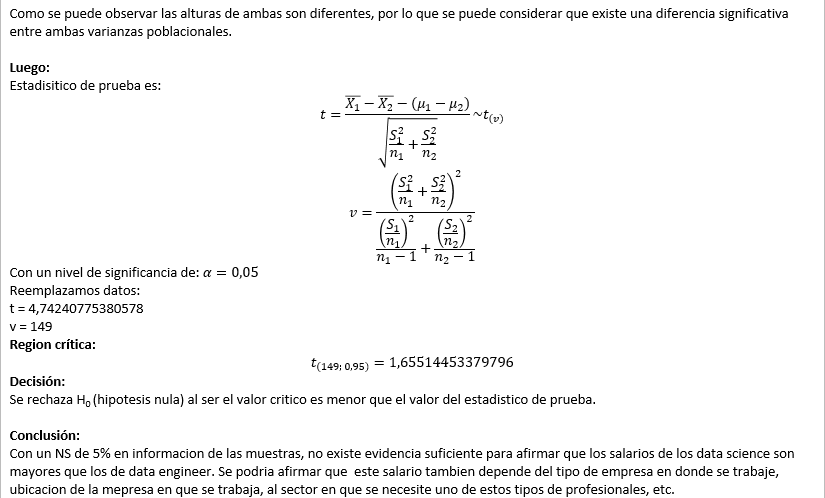
\includegraphics[width=12cm]{Screenshot_20221028_234650.png}
\end{figure}
\end{frame}

\begin{frame}
  \frametitle{Comparacion de salarios publico y privado}
  \[{X_1}: \textrm{Salario publico} \rightarrow \overline{X_1} = 1110.3886, {\sigma_1}^2 = ?\]
  \[{X_2}: \textrm{Salario privado} \rightarrow \overline{X_privado} = 1020.8170, {\sigma_2}^2 = ?\]
\begin{figure}[t]
  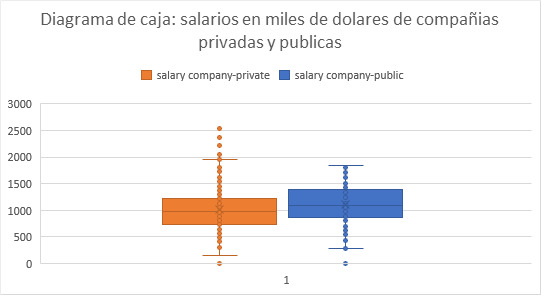
\includegraphics[width=6cm]{cajas2.jpeg}
\end{figure}
\end{frame}

\begin{frame}
  \frametitle{Test de hipotesis}
\begin{figure}[t]
    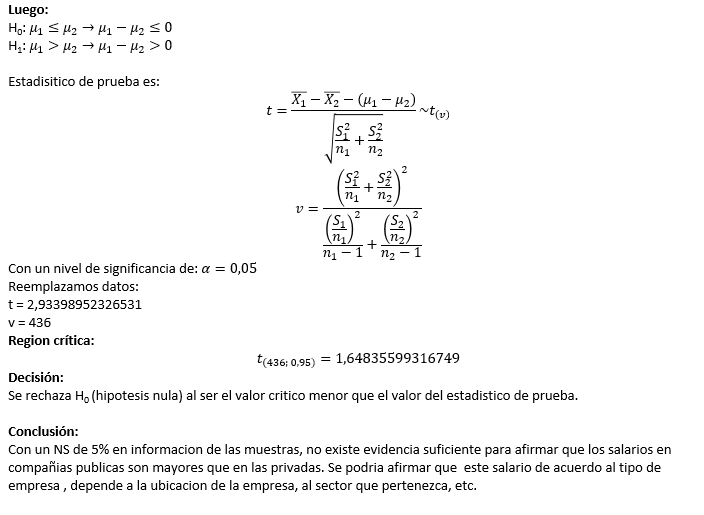
\includegraphics[width=10cm]{Screenshot_20221028_235052.png}
\end{figure}
\end{frame}

\begin{frame}
  \frametitle{Distribucion de ingresos segun edad}
\begin{figure}[t]
    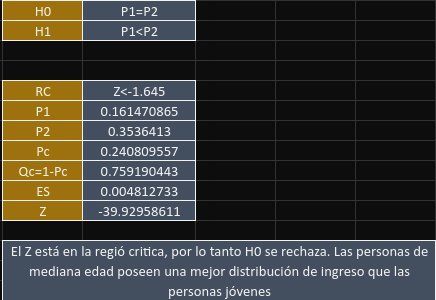
\includegraphics[width=10cm]{cuyate1.png}
\end{figure}
\end{frame}


\begin{frame}
  \frametitle{Distribucion de proporciones ingresos segun edad}
\begin{figure}[t]
    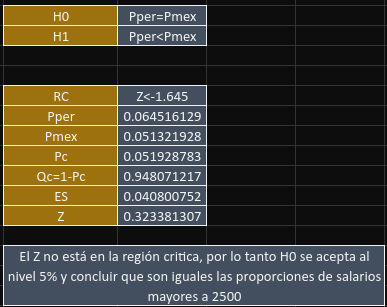
\includegraphics[width=10cm]{cuyate2.png}
\end{figure}
\end{frame}

\begin{frame}
  \frametitle{Comprobar que las personas que trabajan una cantidad
  mayor que la media perciben mejores ingresos
  }
  \begin{figure}[t]
      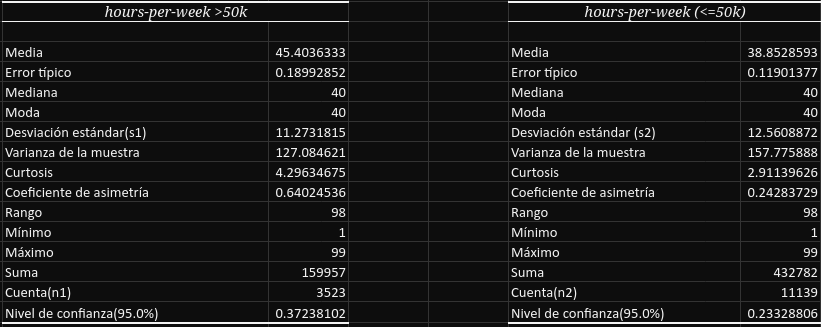
\includegraphics[width=10cm]{alvares1.png}
  \end{figure}
\end{frame}

\begin{frame}
  Para muestras grandes: \[ET = \sqrt{\frac{S_1 ^ 2}{n_1} + \frac{S_2 ^ 2}{n_2}}\]

  \begin{columns}
  \column{0.5\textwidth}
   \[H_0: \mu_1 = \mu_2\]
   \[H_1: \mu_1 > \mu_2\]

  \column{0.5\textwidth}

      \[\textit{Z} = \frac{\overline{X_1} - \overline{X_2}}{ET}\]
      \newline

  \end{columns}

  Dado un error maximo permitido $\alpha = 0.05$, con \textit{$H_1$} indicando una cola unilateral
  hacia la derecha $\rightarrow RC = {Z > 1.645}$

  \[Z_{cal} = \frac{45.4036}{38.8528} = 29.2267\]

  Como \textit{$Z_{cal} \in RC$} Se debe rechazar \textit{$H_0$} y concluir que
  aquellas personas que ganan mas de 50K trabaja en promedio mas que las personas
  que ganan menos de 50K

\end{frame}

\begin{frame}
  \frametitle{Comparar proporciones de trabajadores segun sexo}
  Sean $p_1 \textrm{ y } p_2$ la proporcion de trabajadores femeninos en \textit{Estados Unidos}
  y \textit{Mexico} respectivamente

  Siendo $n_1 = 14662,\textrm{ } x_1 = 4927 \textrm{ y } n_2 = 308, \textrm{ } x_2 = 69$ las cantidades totales
  y de poblacion femenina en ambos paises

  Dando como resultados:

  \[
    \hat{p} = \frac{4927 + 69}{14662 + 308} = 0.3245 \]
  \[
    \textrm{Error tipico: } \overline{p_1} - \overline{p_2}
  \]

  \[
    ET = \sqrt{\frac{\hat{p}(1 - \hat{p})}{n_1} + \frac{\hat{p}(1 - \hat{p})}{n_2}} = 0.02695
  \]

\end{frame}

\begin{frame}

  \begin{columns}
  \column{0.5\textwidth}
   \[H_0: p_1 = p_2\]
   \[H_1: p_1 > p_2\]

  \column{0.5\textwidth}

    Por \textbf{TCL}:
      \[\textit{Z} = \frac{\overline{p}_1 - \overline{p}_2}{ET} \sim N(0, 1)\]
      \newline

  \end{columns}

  Dado un error maximo permitido $\alpha = 0.05$, con \textit{$H_1$} indicando una cola unilateral
  hacia la derecha $\rightarrow RC = {Z > 1.645}$

  \[Z_{cal} = \frac{p_1 - p_2}{ET} = 4.15530\]

  Como \textit{$Z_{cal} \in RC$} Se debe rechazar \textit{$H_0$} y concluir que
  existe una mayor proporcion de mujeres trabajando en ciencia de datos en Estados
  Unidos que en Mexico; sin embargo, ese analisis no puede ser tan confiable debido
  a la diferencia del tamaño de las muestras

\end{frame}

\begin{frame}

  \frametitle{Otras conclusiones}

  \begin{itemize}
    \item Se logra visualizar la formacion de 2 grupos en la poblacion
      de Bangalore independientemente de la variable de analisis

    \item La distribucion teoria a la que mejor se aproximan los ingresos
      es la exponencial, la cual deberia de la distribución \textit{Gamma}

    \item Los test no parametricos son muy suceptibles a :
      \begin{enumerate}
        \item outliers
        \item Distribuciones con ligeras desviaciones de las teoricas
        \item Gran cantidad de data
      \end{enumerate}
  \end{itemize}


\end{frame}

\end{document}
